\section{Text\_\-File\_\-Buffers  Class Reference}
\label{classText__File__Buffers}\index{Text_File_Buffers@{Text\_\-File\_\-Buffers}}
{\tt \#include $<$dil2al.hh$>$}

Inheritance diagram for Text\_\-File\_\-Buffers::\begin{figure}[H]
\begin{center}
\leavevmode
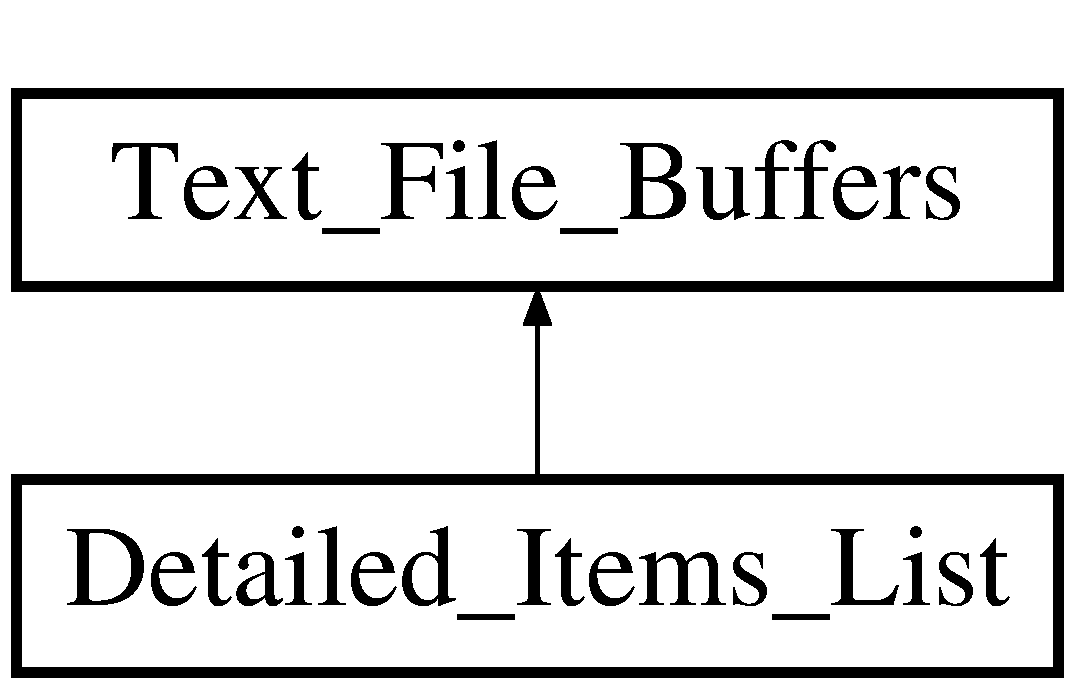
\includegraphics[height=2cm]{classText__File__Buffers}
\end{center}
\end{figure}
\subsection*{Public Methods}
\begin{CompactItemize}
\item 
{\bf Text\_\-File\_\-Buffers} ()
\item 
int {\bf File\-Index} ({\bf String} fname)
\end{CompactItemize}
\subsection*{Public Attributes}
\begin{CompactItemize}
\item 
{\bf String\-List} {\bf tf}
\item 
{\bf String\-List} {\bf tfname}
\item 
int {\bf tfnum}
\end{CompactItemize}


\subsection{Constructor \& Destructor Documentation}
\index{Text_File_Buffers@{Text\_\-File\_\-Buffers}!Text_File_Buffers@{Text\_\-File\_\-Buffers}}
\index{Text_File_Buffers@{Text\_\-File\_\-Buffers}!Text_File_Buffers@{Text\_\-File\_\-Buffers}}
\subsubsection{\setlength{\rightskip}{0pt plus 5cm}Text\_\-File\_\-Buffers::Text\_\-File\_\-Buffers ()\hspace{0.3cm}{\tt  [inline]}}\label{classText__File__Buffers_a0}




Definition at line 205 of file dil2al.hh.

References tfnum.



\footnotesize\begin{verbatim}205 { tfnum=0; }
\end{verbatim}\normalsize 


\subsection{Member Function Documentation}
\index{Text_File_Buffers@{Text\_\-File\_\-Buffers}!FileIndex@{FileIndex}}
\index{FileIndex@{FileIndex}!Text_File_Buffers@{Text\_\-File\_\-Buffers}}
\subsubsection{\setlength{\rightskip}{0pt plus 5cm}int Text\_\-File\_\-Buffers::File\-Index ({\bf String} {\em fname})\hspace{0.3cm}{\tt  [inline]}}\label{classText__File__Buffers_a1}




Definition at line 211 of file dil2al.hh.

References get\_\-file\_\-in\_\-list(), and tfnum.

Referenced by Detailed\_\-Items\_\-List::Write\_\-to\_\-File().



\footnotesize\begin{verbatim}211 { for (int i=0; i<tfnum; i++) if (tfname[i]==fname) return i; return get_file_in_list(fname,tf,tfname,tfnum); }
\end{verbatim}\normalsize 


\subsection{Member Data Documentation}
\index{Text_File_Buffers@{Text\_\-File\_\-Buffers}!tf@{tf}}
\index{tf@{tf}!Text_File_Buffers@{Text\_\-File\_\-Buffers}}
\subsubsection{\setlength{\rightskip}{0pt plus 5cm}{\bf String\-List} Text\_\-File\_\-Buffers::tf}\label{classText__File__Buffers_m0}




Definition at line 207 of file dil2al.hh.

Referenced by Detailed\_\-Items\_\-List::Get\_\-All\_\-DIL\_\-ID\_\-File\_\-Parameters(), Detailed\_\-Items\_\-List::Get\_\-All\_\-Topical\_\-DIL\_\-Parameters(), update\_\-DIL\_\-entry\_\-elements(), and Detailed\_\-Items\_\-List::Write\_\-to\_\-File().\index{Text_File_Buffers@{Text\_\-File\_\-Buffers}!tfname@{tfname}}
\index{tfname@{tfname}!Text_File_Buffers@{Text\_\-File\_\-Buffers}}
\subsubsection{\setlength{\rightskip}{0pt plus 5cm}{\bf String\-List} Text\_\-File\_\-Buffers::tfname}\label{classText__File__Buffers_m1}




Definition at line 208 of file dil2al.hh.

Referenced by Detailed\_\-Items\_\-List::Get\_\-All\_\-DIL\_\-ID\_\-File\_\-Parameters(), Detailed\_\-Items\_\-List::Get\_\-All\_\-Topical\_\-DIL\_\-Parameters(), and update\_\-DIL\_\-entry\_\-elements().\index{Text_File_Buffers@{Text\_\-File\_\-Buffers}!tfnum@{tfnum}}
\index{tfnum@{tfnum}!Text_File_Buffers@{Text\_\-File\_\-Buffers}}
\subsubsection{\setlength{\rightskip}{0pt plus 5cm}int Text\_\-File\_\-Buffers::tfnum}\label{classText__File__Buffers_m2}




Definition at line 209 of file dil2al.hh.

Referenced by File\-Index(), Detailed\_\-Items\_\-List::Get\_\-All\_\-DIL\_\-ID\_\-File\_\-Parameters(), Detailed\_\-Items\_\-List::Get\_\-All\_\-Topical\_\-DIL\_\-Parameters(), Text\_\-File\_\-Buffers(), and update\_\-DIL\_\-entry\_\-elements().

The documentation for this class was generated from the following file:\begin{CompactItemize}
\item 
{\bf dil2al.hh}\end{CompactItemize}
